% Chapter Template

\chapter{MODI} % Main chapter title

\label{Chapter3} % Change X to a consecutive number; for referencing this chapter elsewhere, use \ref{ChapterX}

\lhead{Capítulo 3. \emph{MODI}} % Change X to a consecutive number; this is for the header on each page - perhaps a shortened title

%----------------------------------------------------------------------------------------
%	SECTION 1
%----------------------------------------------------------------------------------------

\begin{figure}[htbp]
	\centering
		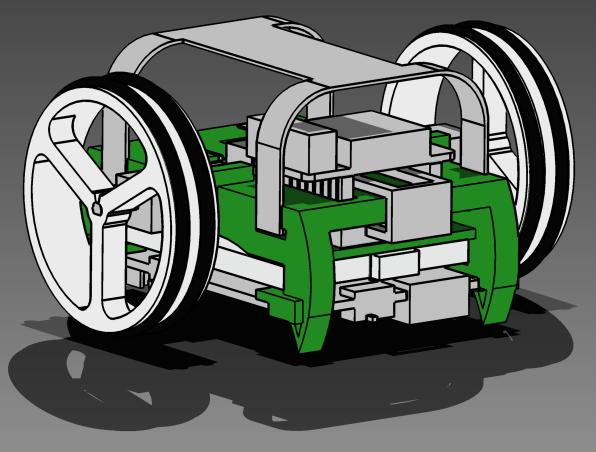
\includegraphics[width=0.8\textwidth]{./Figures/MODI/render.png}
		\rule{35em}{0.5pt}
	\caption[modi]{robot MODI (sigla para Modular Intelligence)}
	\label{fig:MODI}
\end{figure}

\section{Setup}

Se desea realizar una investigación sobre el comportamiento colectivo de un grupo de robots, en el mundo real sin hacer uso de simuladores. Por esto  es necesario contar con un lugar físico donde poder activar los robot. Además para simplificar cada uno de los robots, estos no tienen sensores internos por lo que hay una cámara montada sobre el plano de movimiento de estos, para hacer Seguimiento Visual.
\begin{figure}[htbp]
	\centering
		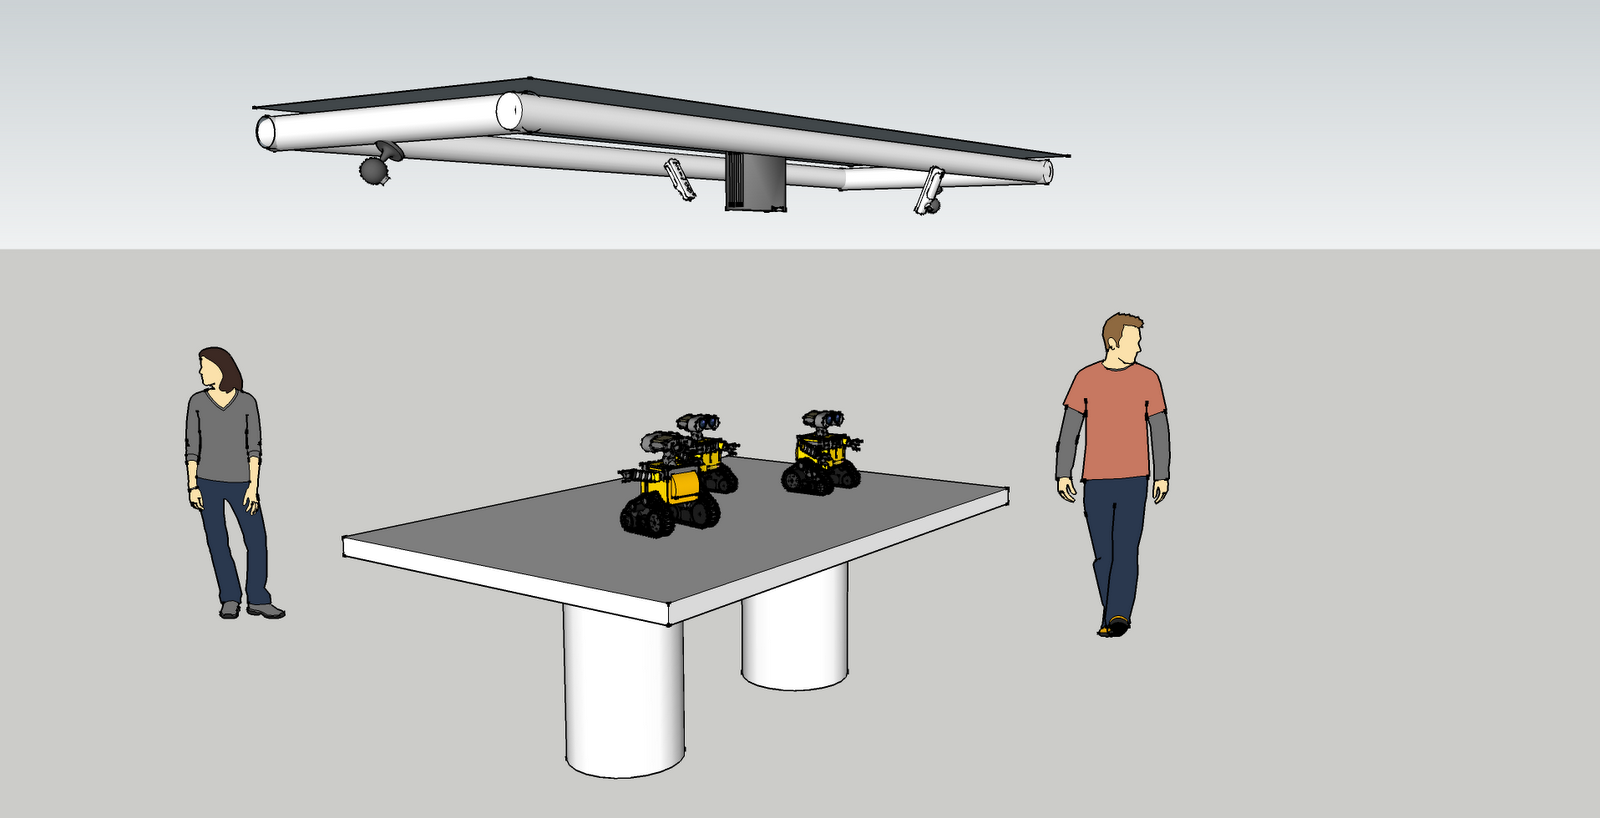
\includegraphics[width=0.8\textwidth]{./Figures/setup.png}
		\rule{35em}{0.5pt}
	\caption[Setup]{Setup a montarse para hacer estudios de grupos de robots.}
	\label{fig:setup}
\end{figure}

La función principal de MODI es ser una plataforma móvil de fácil acceso. Existe un repositorio en GitHub donde se tienen los códigos actualizados para controlar y construir robots MODI.  Para descargar códigos y piezas de construcción se debe ir a github.com/FabLabUCh/modi

\textbf{Las funciones principales que se desarrollaron}

\begin{itemize}
\item Carga Autónoma con celda solar.
\item Seguimiento de grupo.
\item Control individual del color de cada MODI.
\item Movimiento simple de cada robot de forma independiente.
\end{itemize}


%-----------------------------------
%	SECTION 2
%-----------------------------------

\section{Construcción}

%-----------------------------------
%	SUBSECTION 2
%-----------------------------------
\subsection{Fabricación Digital vs Análoga}
Cuando se quiere pasar una idea al mundo real es necesario un proceso de fabricación. Dependiendo de la cantidad de herramientas que se tenga es más o menos fácil la tarea. Desde el comienzo hasta hace un par de años, quienes se dedican a construir robots, debían construir de manera “artesanal” donde es imposible que las piezas queden todas iguales y el tiempo empleado era bastante. Hoy en día existe una gran alternativa que surge como un nuevo paradigma, la Fabricación Digital. Las impresoras 3D, que no son más que un extrusor montado en un sistema con ejes que le dan 3 grados de libertad, permiten desde un modelo hecho en un computador, obtener un objeto real en plástico. También existe otro tipo de máquinas que permite hacer diseños en 2D, estas son las cortadoras LASER. La primera versión de MODI fue construido usando planchas de madera MDF y acrílico, cortados en LASER.




Utilizando una impresora 3D Makerbot Replicator 1 se hizo esta primera versión con piezas plásticas.

\begin{figure}[htbp]
	\centering
		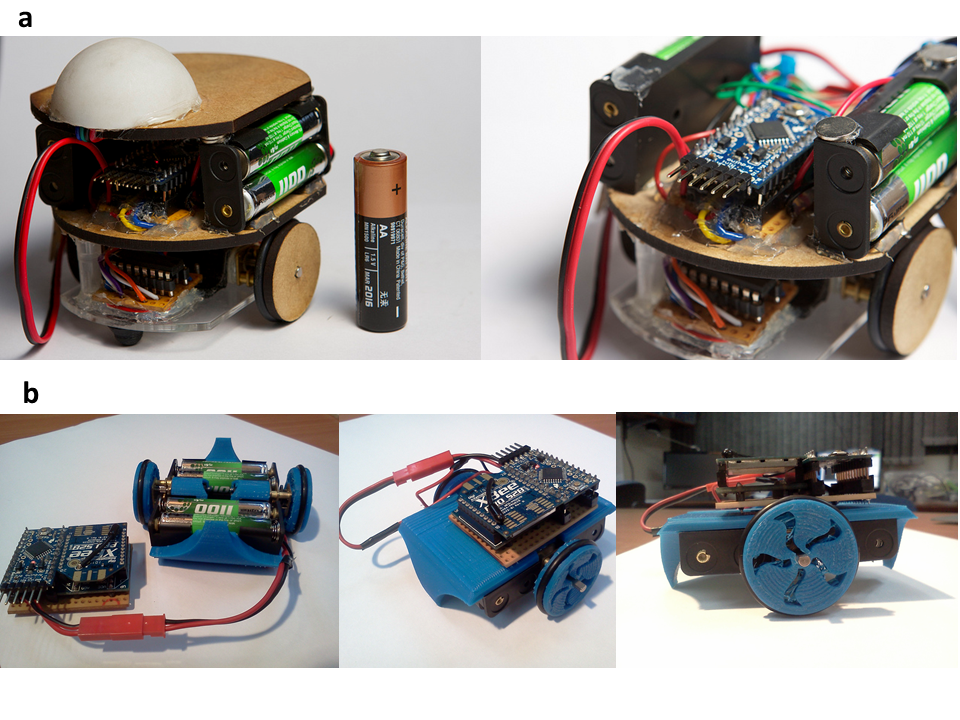
\includegraphics[width=0.8\textwidth]{./Pictures/modi_analogToDigital.png}
		\rule{35em}{0.5pt}
	\caption[modireplicator]{Primera versión de MODI usando técnica de \emph{ Fabricación Digital }con chasis de plástico construido con una MakerBot Replicator 1}
	\label{fig:modireplicator}
\end{figure}



Esta versión se dio de baja ya que presentaba el problema de involucrar demasiadas partes que debían ser hechas por una persona. El microcontrolador, junto con la radio inalámbrica se colocaron en una placa electrónica para prototipado, más adelante se puede ver que fueron reemplazados por una PCB llamada Arduino FIO, que es una plataforma de desarrollo Arduino junto con un socket Xbee. Otro factor clave para descartar esta versión es que utiliza 4 pilas AAA que necesitan ser removidas para poder ser recargadas, lo que impide que en futuras versión exista la posibilidad de una carga autónoma por parte de los Robots. La versión actual de modi permite su carga por medio de un puerto Mini USB, panel solar y de forma inalámbrica.

Aunque han bajado los precios de las maquinas para prototipado rápido, aún no están al alcance de todas las personas. Es por esto que existen los Fab Labs (acrónimo del inglés Fabrication Laboratory), que según Wikipedia es, \textit{un espacio de producción de objetos físicos a escala personal o local que agrupa máquinas controladas por ordenadores. Su particularidad reside en su tamaño y en su fuerte vinculación con la sociedad.} Los Fab Labs están por todo el mundo, Figura \ref{fig:Fablabs}. MODI fue concebido como un proyecto del Fab Lab de la Universidad de Chile y por esto es posible reproducirlo en cualquier Fab Lab. En Chile, además del Fab Lab de la Universidad de Chile están: Design LAB UAI, Fab Lab Santiago y Stgo MakerSpace. 

\begin{figure}[htbp]
	\centering
		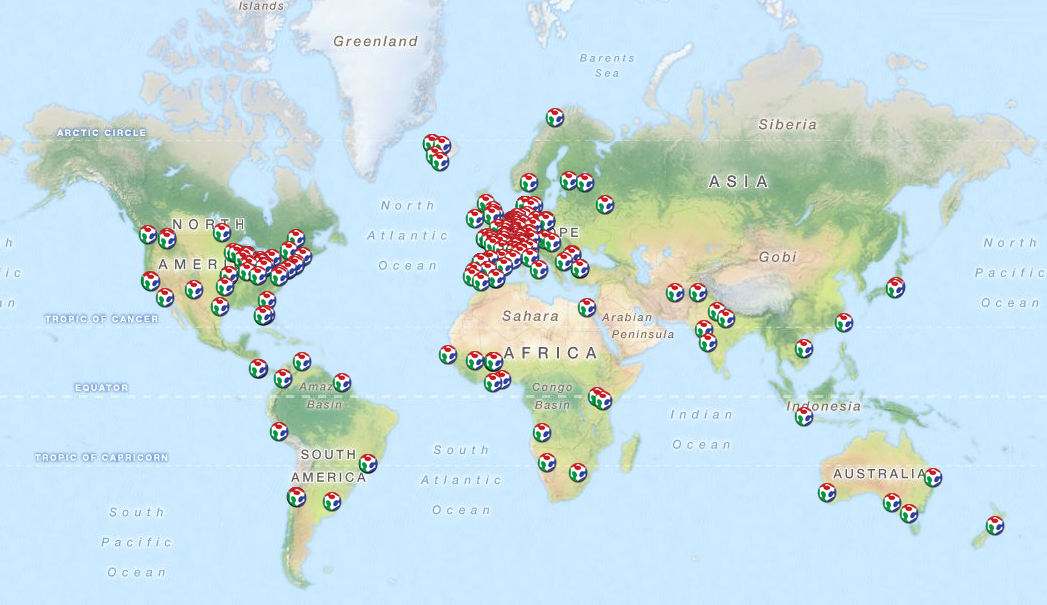
\includegraphics[width=0.8\textwidth]{./Figures/map.png}
		\rule{35em}{0.5pt}
	\caption[Fablabs]{Mapa actual de lugares en el mundo que cuentan con un Fab Lab. En Chile a la fecha existen 3. Imagen obtenida desde fablabamersfoort.nl/fablabs/}
	\label{fig:Fablabs}
\end{figure}	

%-----------------------------------
%	SUBSECTION 3
%-----------------------------------
\subsection{Software CAD}

CAD viene de sus siglas del Inglés, Computer-aided design, y se refiere a un diseño asistido por herramientas computacionales. Profesionales como ingenieros, arquitectos y del área del diseño por lo general son los que hacen más uso de estas herramientas.

Según Wikipedia, \textit{”... se pueden dividir básicamente en programas de dibujo en dos dimensiones (2D) y modeladores en tres dimensiones (3D). Las herramientas de dibujo en 2D se basan en entidades geométricas vectoriales como puntos,líneas, arcos y polígonos, con las que se puede operar a través de una interfaz gráfica....”}

Durante el transcurso del proyecto se trabajó con varios softwares CAD. El primero fué SketchUp 8 de Google, que permite fácilmente hacer bocetos de lugares y cuenta con una importante biblioteca de modelos para incluir en el diseño. Rápidamente se pudo hacer un scketch utilizando modelos descargados de Internet , Figura~\ref{fig:setup}.

El diseño del chasis junto con las ruedas y demás partes plásticas, se hizo en un comienzo con SolidWorks 2012 y luego por ser más simple de usar, Inventor 2013 de Autodesk. Ambos softwares permiten generar modelos en 3D para luego exportar el diseño al formato STL que es estándar para prototipar en plástico.


\begin{figure}[htbp]
	\centering
		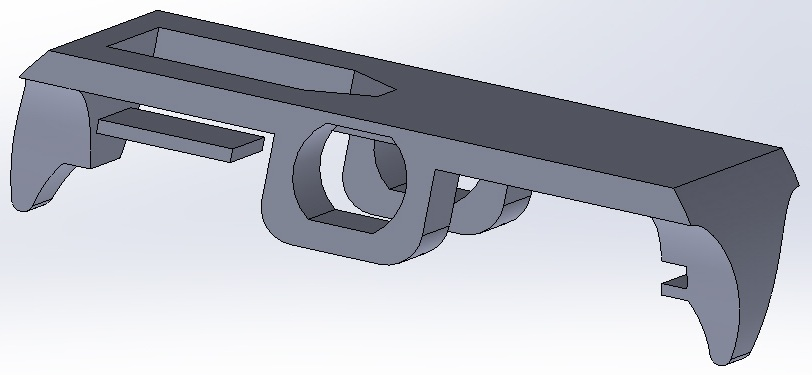
\includegraphics[width=0.9\textwidth]{./Figures/MODI/1MODI.jpg}
		\rule{35em}{0.5pt}
	\caption[ModiSolidWorks]{Primer Chasis de MODI, realizado con SolidWorks 2012. Esta versión sirve solo como prueba de concepto ya que no tiene espacio para las conexiones eléctricas necesarias}
	\label{fig:MODISolidWork}
\end{figure}	

Luego de varias iteraciones se lográ este modelo, Figura \ref{fig:render3} que tiene cinco piezas. 


\begin{figure}[htbp]
	\centering
		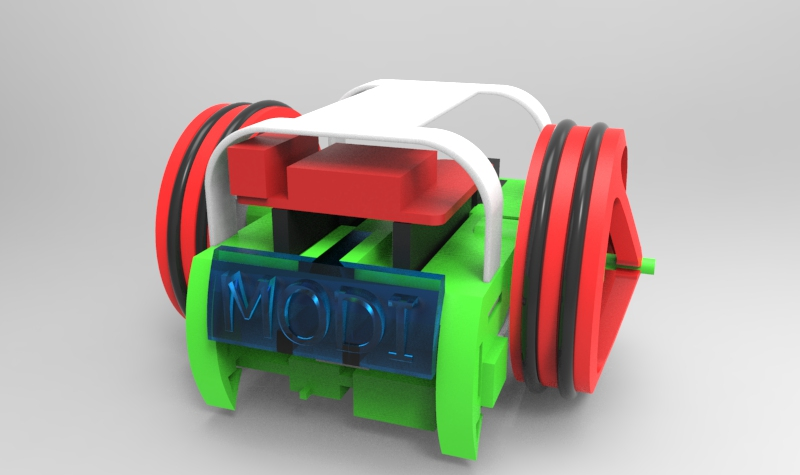
\includegraphics[width=0.9\textwidth]{./Figures/MODI/render3.jpg}
		\rule{35em}{0.5pt}
	\caption[Render modi]{Modelos 3D de MODI realizado con Autodesk Inventor 2013 y renderizado con KeyShot4. }
	\label{fig:render3}
\end{figure}	


%-----------------------------------
%	SUBSECTION 4
%-----------------------------------
\subsection{Impresora 3D} \label{cap:impresora3D}

Parte importante de este trabajo se realizó con impresoras 3D. Estas existen desde los años 80' y hasta hace algunos años por su precio y tamaño eran de dificil acceso. Utilizan distintas tecnologías, las que se utilizaron en el proceso de este trabajo son las FDM, sigla del ingles "Fused deposition modeling" donde un cabezal extrusor de plástico se mueve en el plano xy depositando capa por capa de material mientras avanza en el eje z.

\begin{figure}[htbp]
	\centering
		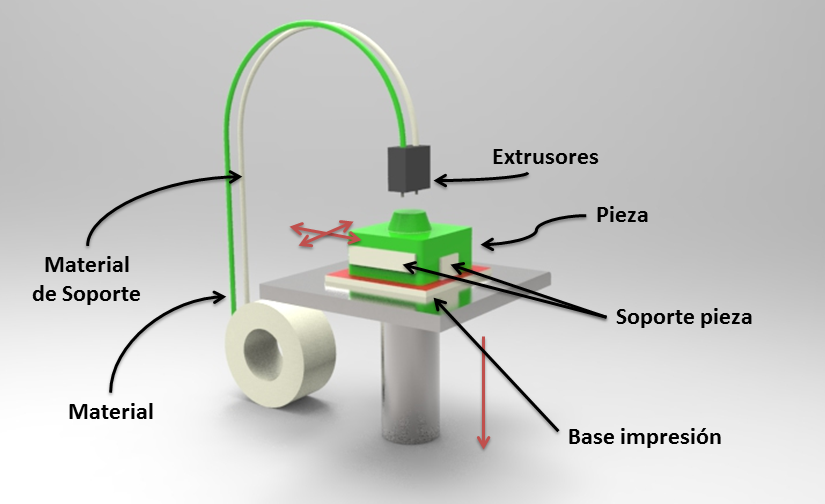
\includegraphics[width=0.8\textwidth]{./Figures/3Dprint.png}
		\rule{35em}{0.5pt}
	\caption[3Dprint]{Modelo de funcionamiento para impresoras 3D MDF. Tiene dos materiales, uno para construir la pieza y otro que funciona como soporte estructural para la impresión, además existe una base que se calienta para sujetar la pieza mientras se construye.}
	\label{fig:3Dprint}
\end{figure}	

Primero se utilizó la 3D Touch Dual de la empresa Bit from Bytes, que permite hacer modelos de hasta 185 x 273 x 200[mm], con una buena resolución de 0.125[mm]\footnote{teambastech.com/Store/index.php?route=product/product\&product\_id=205} cada capa en eje z. Luego por facilidad de uso y menor tiempo de impresión se usa una impresora MakerBot Replicator 1

\begin{table}\small 
    \begin{tabular}{l|lll}
    ~                     & Replicator 1                          & 3D Touch                   & Uprint      \\ \hline
    Volumen impresión         & 5$ m^{3} $                            & 10 $m^{3}$                 & 4.7 $m^{3}$ \\
    Espesor capa      & 0.3 mm                                & 0.125mm                    & 0.254 mm    \\
    Velocidad                 & 40 mm/s                               & 6 mm/s                     & lenta       \\
    Precisión & 2.5 $ \mu $m Z , 11$\mu$m XY  & 0.1mm Z  0.2mm XY  & ~           \\
    Material soporte  & con herramienta &con herramienta  & Necesita proceso extra      \\
    Precio insumo   &60USD/Kg	                          &           100USD/Kg         & 400USD/Kg        \\
    
    \end{tabular}
    \caption {Comparación impresoras 3D}
\end{table}

\begin{figure}[htbp]
	\centering
		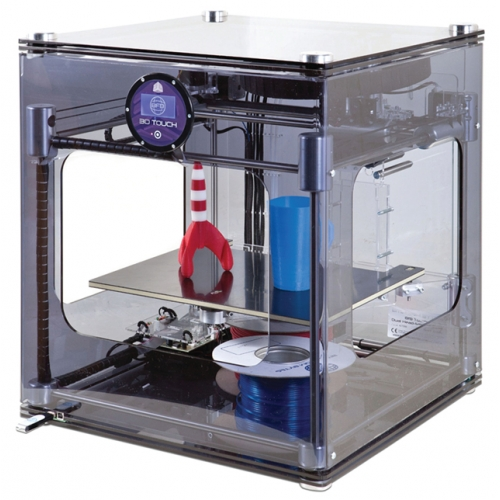
\includegraphics[width=0.6\textwidth]{./Figures/3dtouch.jpg}
		\rule{35em}{0.5pt}
	\caption[3DTouch]{Impresora 3D de Bit From Bytes, 3D Touch.}
	\label{fig:3Dtouch}
\end{figure}	

\begin{figure}[htbp]
	\centering
		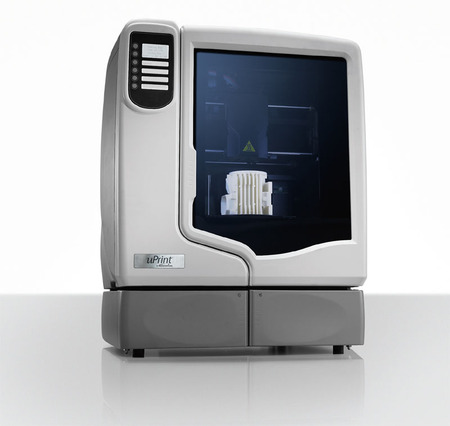
\includegraphics[width=0.6\textwidth]{./Figures/uprint.jpg}
		\rule{35em}{0.5pt}
	\caption[uprint]{Impresora 3D de Stratasys, Uprint SE.}
	\label{fig:uprint}
\end{figure}	


\begin{figure}[htbp]
	\centering
		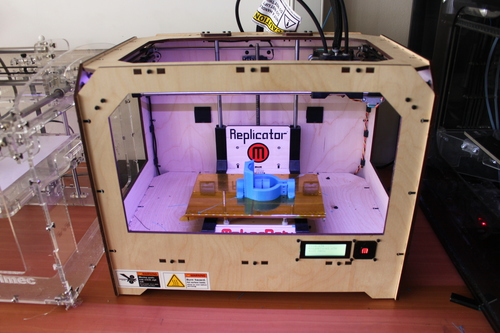
\includegraphics[width=0.6\textwidth]{./Figures/replicator1.jpg}
		\rule{35em}{0.5pt}
	\caption[Replicator1]{Replicator 1 de Makerbot, impresora 3D FDM utilizada para prototipar chasis y ruedas de robot MODI. En Laboratorio de Síntesis de maquinas inteligentes de la Universidad de Chile, junto a la Fab@Home y 3DTouch.}
	\label{fig:replicator}
\end{figure}	


\newpage

%-----------------------------------
%	SUBSECTION 5
%-----------------------------------
\subsection{Diseño PCB}


\begin{figure}[htbp]
	\centering
		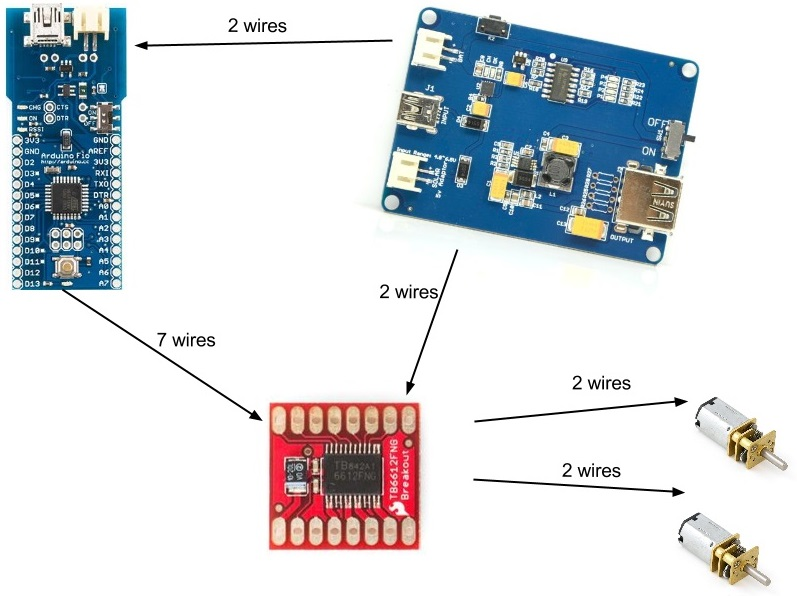
\includegraphics[width=0.8\textwidth]{./Figures/Diagrama.jpg}
		\rule{35em}{0.5pt}
	\caption[cables]{15 conexiones que unen distintos componente.}
	\label{fig:Diagrama cables}
\end{figure}	

En los primeros prototipos un problema que se repetía constantemente son las conexiones entre los sistemas que componen al robot. Son 15 conexiones que unen distintos componentes, Figura \ref{fig:Diagrama cables}. Por esto es necesario un PCB que permita reducir al mínimo el espacio necesario para para energizar y comunicar los elementos. El requerimiento principal es poder fabricarse con una fresa CNC como la Roland Modela MDX-20, por lo que es necesario diseñar un PCB de una sola capa. Se utilizó Eagle como software para el diseño del diagrama eléctrico y PCB, el resultado se puede ver en la Figura \ref{fig:pcbeagle}.

\begin{figure}[htbp]
	\centering
		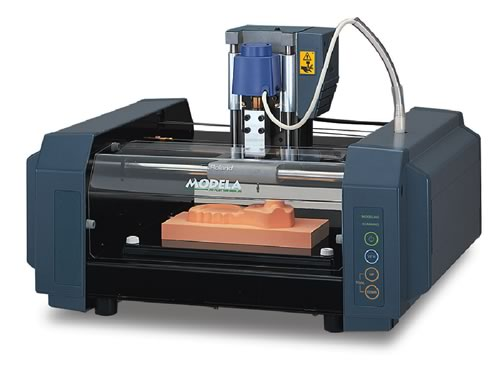
\includegraphics[width=0.5\textwidth]{./Pictures/MDX20.jpg}
		\rule{35em}{0.5pt}
	\caption[MDX20]{Roland Modelo MDX-20 usada para hacer PCB y modelos 3D. Imagen tomada de roland.com}
	\label{fig:MDX20}
\end{figure}

\begin{figure}[htbp]
	\centering
		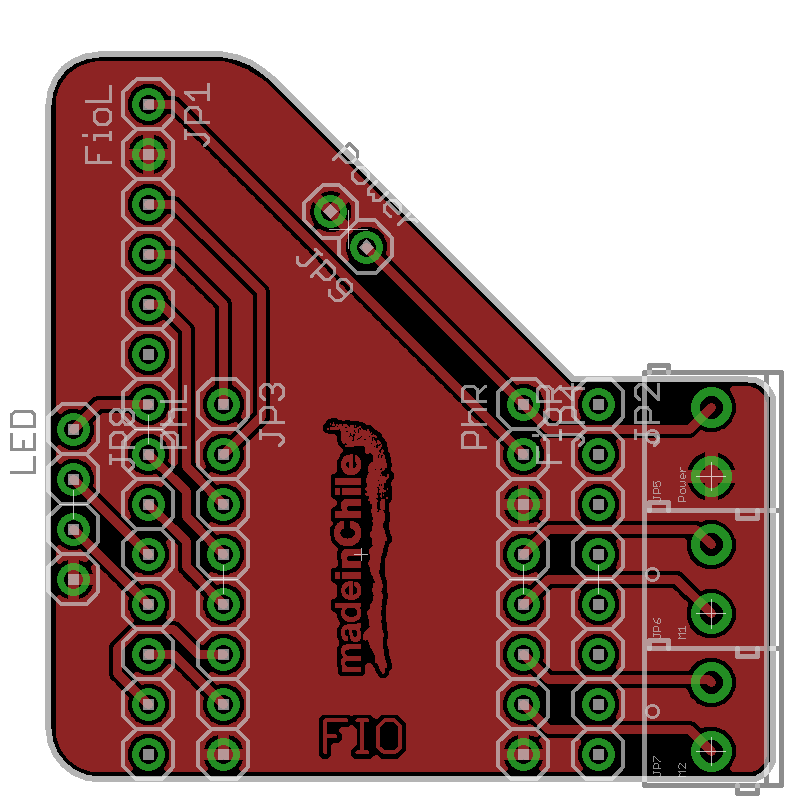
\includegraphics[width=0.5\textwidth]{./Figures/MODI/pcbmodi.png}
		\rule{35em}{0.5pt}
	\caption[pcbeagle]{MODIBoard es una PCB diseñada para poder conectar de forma simple los diversos componentes electrónicos. Conecta: Arduino Fio, Lipo Rider Pro, Motor Driver, LED RGB y Motores.}
	\label{fig:pcbeagle}
\end{figure}

\begin{figure}[htbp]
	\centering
		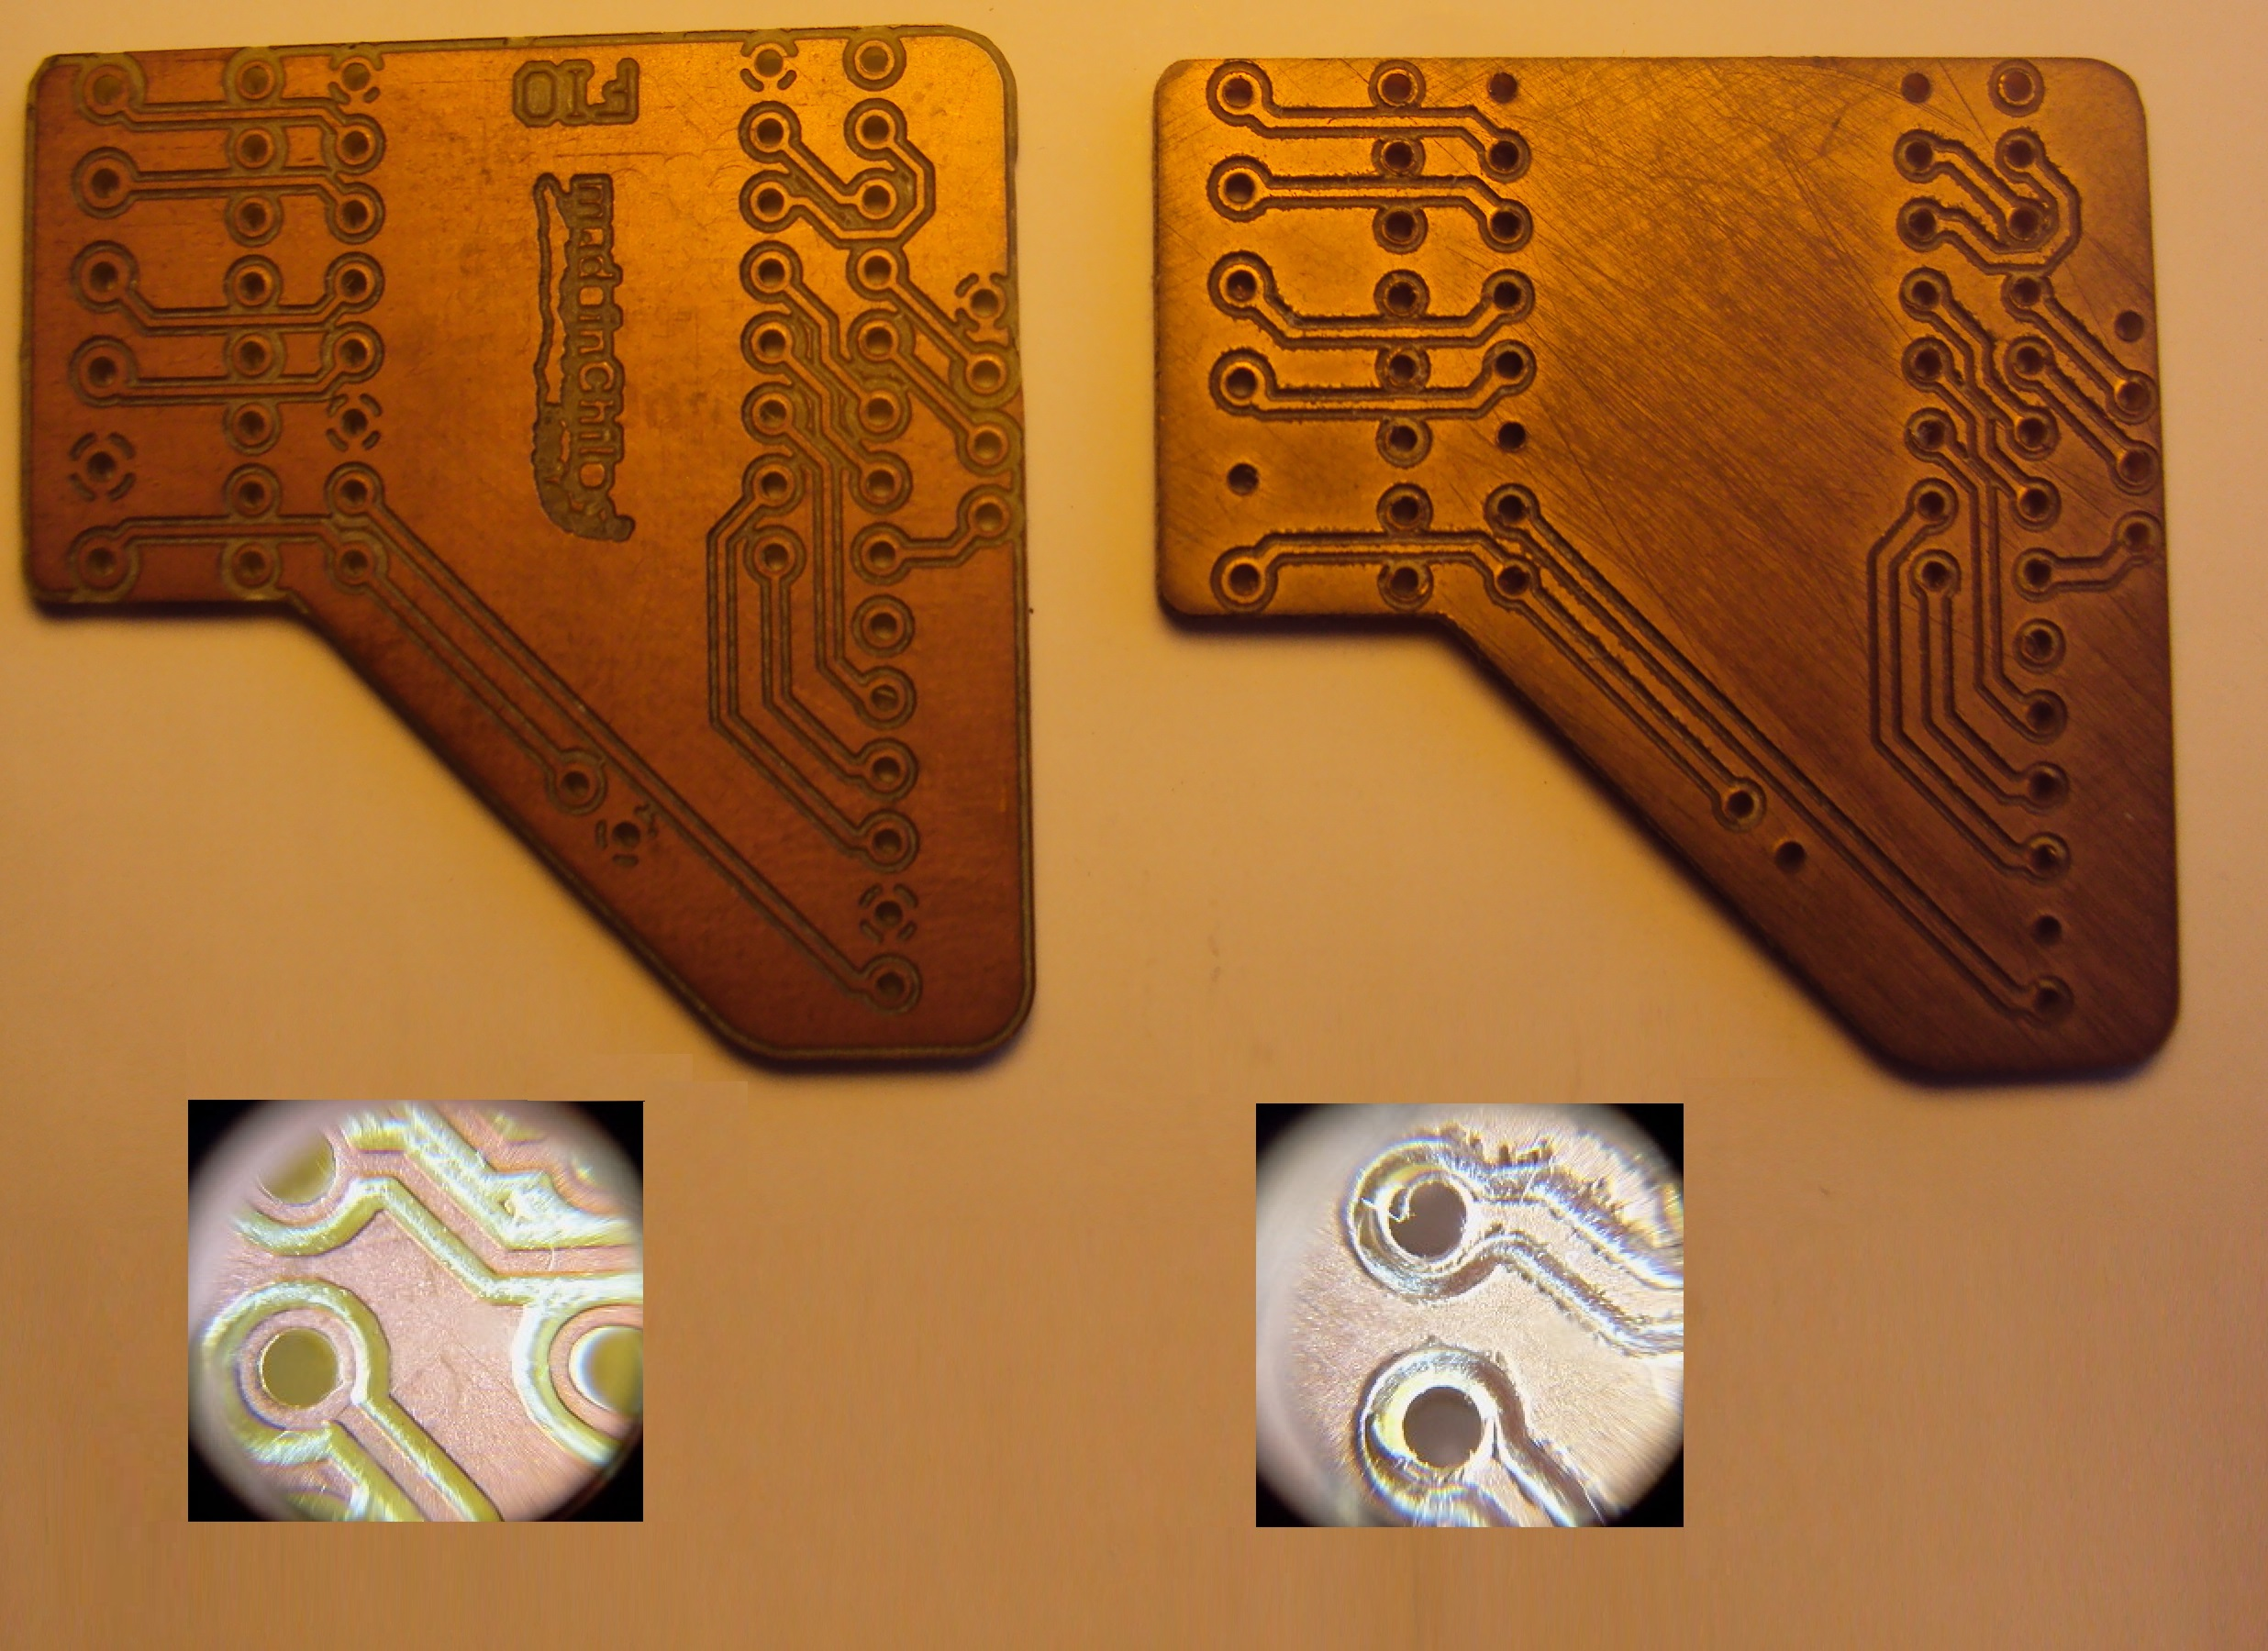
\includegraphics[width=0.8\textwidth]{./Pictures/pcb.jpg}
		\rule{35em}{0.5pt}
	\caption[pcb]{Misma PCB fresada en dos maquinas diferentes. Se puede apreciar en el detalle aumentado 60x, la importancia de contar con una buena resolución de fresado. En especial es necesario para tener un buen pad.}
	\label{fig:pcb}
\end{figure}
%-----------------------------------
%	SECTION 2
%-----------------------------------

\section{Componentes electrónicos}

MODI está compuesto por varios componentes electrónicos que implementan tecnologías nuevas. De forma sencilla el usuario puede hacer uso de todas estas, que por ser Open Source tienen una amplia documentación. Su uso en colegios, talleres y universidades, por ser de bajo costo, y sin partes externas extremadamente frágiles, es una excelente herramienta para iniciar a alumnos en temas como la Programación, Robótica, Comunicación Inalámbrica y Visión Artificial, entre otros, sin los miedos asociados a utilizar un equipo costoso y delicado.

El robot MODI es pequeño y de fácil construcción con las herramientas de Fabricación Digital que se puede encontrar en un FabLab. Tiene un pequeño microcontrolador \textbf{Arduino} que controla dos motores, y un \textbf{XBee} para la comunicación inalámbrica con un computador central que usando cualquier lenguaje de programación con comunicación serial puede controlar uno o más robots. La posición de cada robot se obtiene con tags \textbf{Fiduciales}, que permiten por medio de una cámara cenital saber la coordenada y rotación de cada uno. En esta primera aplicación es necesario contar con autonomía energética por lo que se incluye una batería lipo de 2000[mAh] junto a un módulo que carga la batería y eleva el voltaje de salida a 5[v]. Este el módulo de carga, \textbf{Lipo Rider Pro}, tiene además la ventaja de permitir distintos tipos de carga, como una celda de carga solar o un sistema de carga inalámbrica por medio de bobinas. Tener la posibilidad de cargar una batería con luz solar o por medio de forma inalámbrica hace posible el hacer experimentos que necesiten estar funcionando semanas sin la intervención de un humano para cargar cada uno.

%-----------------------------------
%	SUBSECTION 1
%-----------------------------------
\subsection{Arduino FIO}

Microcontrolador
El Arduino FIO ha sido diseñado por Shigeru Kobayashi, es una placa para microcontrolador basada en el ATmega328P. Funciona a 3.3V y 8 MHz. Tiene 14 pines de I/O digitales (de los cuales 6 pueden usarse como salidas PWM), 8 entradas analógicas, un oscilador en placa, un botón de reinicio (reset), y agujeros para montar conectores de pines. Tiene conexiones para una batería de polímero de Litio e incluye un circuito de carga a través de USB. En el reverso de la placa tiene disponible un zócalo para módulos XBee.

El Arduino FIO está diseñado para aplicaciones inalámbricas. El usuario puede subir sus sketches con un cable FTDI o una placa adicional adaptadora Sparkfun. Además, si utiliza un adaptador de USB a XBee modificado (como el USB Explorador de XBee), el usuario puede subir sketches de forma inalámbrica. La tarjeta viene sin conectores pre-montados, permitiendo el uso de diversos tipos de conectores o la soldadura directa de los cables. La tabla \ref{table:Especificaciones Fio} resume sus características principales.

Arduino FIO. Similar al arduino mini pro pero además incluye conexión para módulo XBee. Imagen tomada de arduino.cc


\begin{figure}[htbp]
	\centering
		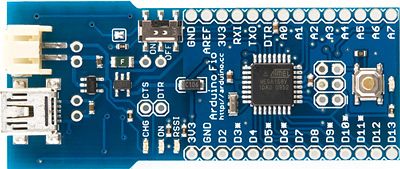
\includegraphics[width=0.8\textwidth]{./Figures/MODI/fio.jpg}
		\rule{35em}{0.5pt}
	\caption[fio]{Arduino FIO. Similar al arduino mini pro pero además incluye conexión para módulo XBee. Imagen tomada de arduino.cc}
	\label{fig:fio}
\end{figure}

\begin{table}
    \begin{tabular}{l|l}
    Microcontrolador             & ATmega328P                             \\
    Voltaje operación            & 3.3 V                                  \\
    Input Vontaje                & 3.35 - 12 V                            \\
    Input Voltaje carga batería  & 3.7 - 7 V                              \\
    Pins Digital I/O             & 14 (con 6  salidas PWM)                \\
    Input Pins Analogos          & 8                                      \\
    Corriente DC en cada Pin I/O & 40 mA                                  \\
    Memoria Flash                & 32 KB (2KB son usados para Bootloader) \\
    SRAM                         & 2 KB                                   \\
    EEPROM                       & 1 KB                                   \\
    Clock                        & 8 MHz                                  \\
    \end{tabular}
    \caption[Especificaciones Fio]{Especificacion tecnica de Arduiono FIO}
	\label{table:Especificaciones Fio}
\end{table}

\begin{figure}[htbp]
	\centering
		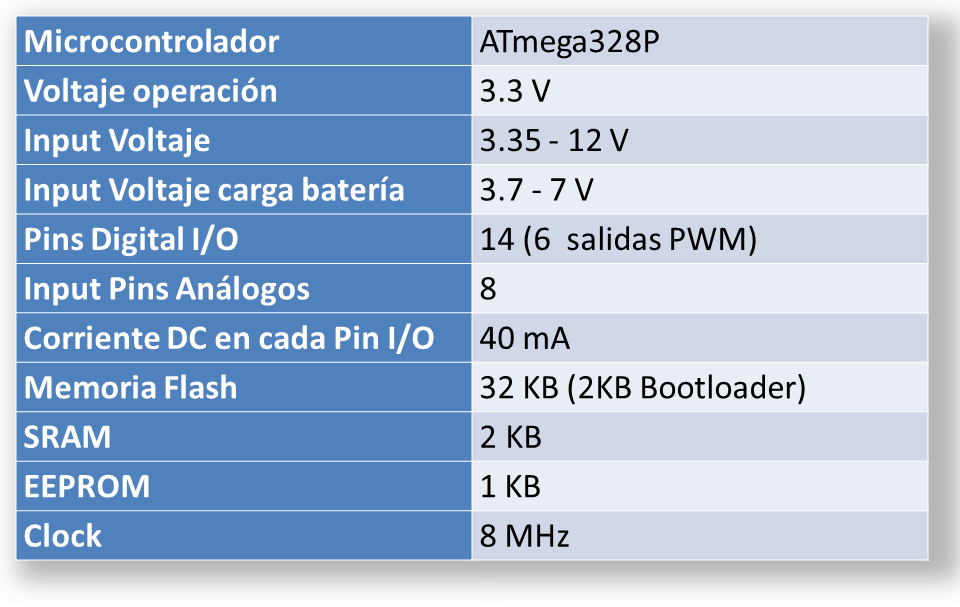
\includegraphics[width=0.6\textwidth]{./Figures/MODI/fio.png}
		\rule{35em}{0.5pt}
	\caption[fio]{Arduino FIO. Similar al arduino mini pro pero además incluye conexión para módulo XBee. Imagen tomada de arduino.cc}
	\label{fig:fio1}
\end{figure}

\begin{figure}[htbp]
	\centering
		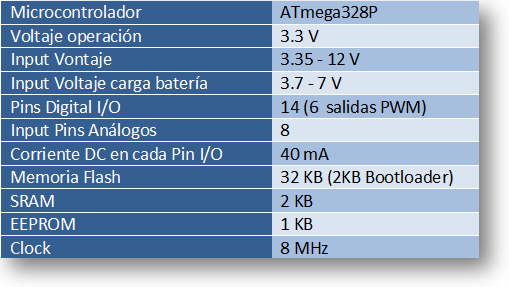
\includegraphics[width=0.6\textwidth]{./Figures/MODI/fio2.png}
		\rule{35em}{0.5pt}
	\caption[fio]{Arduino FIO. Similar al arduino mini pro pero además incluye conexión para módulo XBee. Imagen tomada de arduino.cc}
	\label{fig:fio2}
\end{figure}

%-----------------------------------
%	SUBSECTION 2
%-----------------------------------
\subsection{Motores DC}

Este motor Pololu es muy pequeño (largo: 9.27 mm), por lo mismo usa muy poca corriente. Además tiene una caja de reduccion metalica de 30:1. El eje tiene forma de D.

Pese a no ser la alternativa más económica, estos motores han sido muy difundidos para su uso en robótica por su bajo consumo y alto torque. La tabla \ref{table:Motor} resume sus características principales.

\begin{figure}[htbp]
	\centering
		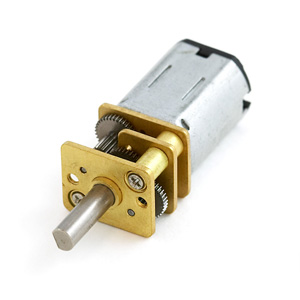
\includegraphics[width=0.5\textwidth]{./Figures/MODI/Motorpololu.jpg}
		\rule{35em}{0.5pt}
	\caption[MotorDC]{Motor pololu con reducción 1:30. Imagen tomada de pololu.com}
	\label{fig:MotorDC}
\end{figure}

\begin{table}
    \begin{tabular}{l|l}
    Velocidad &  440 RPM @6 V, 40 mA\\
    Torque                & 3 Kg-mm  \\
    Reducción             & 1:30     \\
    Consumo trancado      & 0.36 A   \\
    \end{tabular}
        \caption[Motor]{Especificación técnica de Motor DC Pololu}
	\label{table:Motor}
\end{table}

%-----------------------------------
%	SUBSECTION 3
%-----------------------------------
\subsection{XBee}

Los dispositivos con los cuales interactuamos a diario poseen acceso a distintos tipos de sistemas de comunicación. Los llamados “Smartphone” cuentan con diversas antenas para conectarse, WIFI, Bluetooth, red celular,  por nombrar algunas. Estamos en un momento en que las comunicaciones son una de las claves tecnológicas que nos permiten cumplir con tareas que para nuestros abuelos eran imposibles de hacer en un día. Es claro que un sistema con varios o cientos de robots también necesitan comunicarse. 

Para comunicar un robot con otro pueden usarse diversas técnicas. Dependiendo del área en particular que sea del interés del científico, los robot pueden comunicarse por medio de sensores de proximidad o tacto, para saber que hay otro cerca, pueden tener un sistema de visión artificial con una cámara a bordo que le permita “ver” el entorno al robot, con parlantes y micrófonos pueden emitir algún ruido que sea interpretado por su entorno, o lo mismo con sensores de otros tipos.

El robot que se construyó para hacer las pruebas cuenta con un sistema externo de visión artificial que permite obtener posición y orientación de cada robot. Esta información es transmitida a cada robot por medio del protocolo zigbee implementado en los chip XBee de la empresa Digi, Figura \ref{fig:xbee}. Esto permite comunicar un alto número de robots, con muy poco consumo energético y de manera relativamente simple. Se escogió usar visión artificial sobre el sistema para bajar los costos individuales de los robots y XBee por ser el estándar en la industria en redes de sensores inalámbricos. Cabe destacar que los robots que existen en el mercado no incluyen XBee, y los que lo traen lo hacen como accesorio. 


\begin{figure}[htbp]
	\centering
		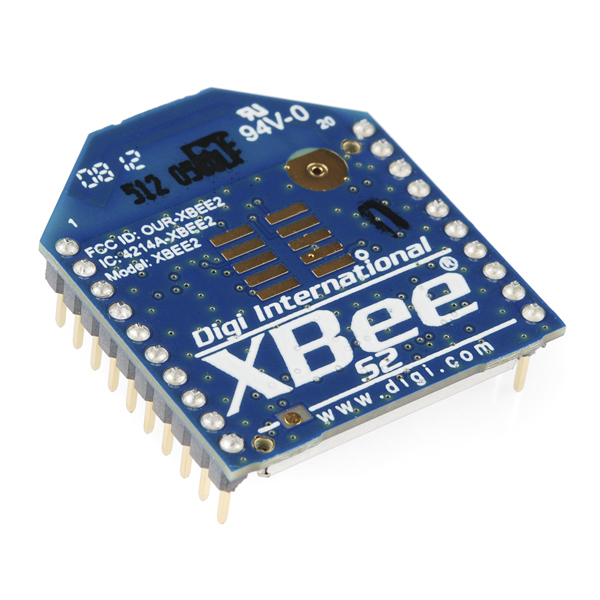
\includegraphics[width=0.5\textwidth]{./Figures/MODI/xbee.jpg}
		\rule{35em}{0.5pt}
	\caption[xbee]{Xbee es un producto de la empresa Digi basado en el conocido protocolo de comunicación inalámbrica ZigBee. El módulo Xbee XBP24-AWI-001 funciona a 2.4GHz. La serie Pro tiene el mismo pinout y set de instrucciones que la serie básica más un incremento de la potencia de salida a 60mW. Estos módulos permiten extender la comunicación serial de forma inalámbrica.
Con Xbee se pueden hacer redes punto a punto y multipunto de forma fácil.}
	\label{fig:xbee}
\end{figure}

3.3V @ 295 mA.
Tasa de datos máximo de 250kbps.
50mW de salida (+17dBm).
1600m de rango.
Antena interna.
Certificado total FCC.
4 pines de entrada de 10-bit ADC.
10 pines digitales de Entrada/Salida.
Encriptación en 128 bit.
Configuración local o ‘en el aire’.
Set de comandos AT o API.




%-----------------------------------
%	SUBSECTION 3
%-----------------------------------
\subsection{Lipo Rider Pro}

El LiPo Rider Pro es una versión mejorada del LiPo Rider, que es una fuente de poder para alimentar distintos gadget con energía verde. Esta placa permite alimentar con 5V distintos dispositivos. Puede obtener energía del sol o por medio de inducción magnética. También puede cargar un SmartPhone. Figura \ref{lipopro1}
\newpage

\begin{figure}[htbp]
	\centering
		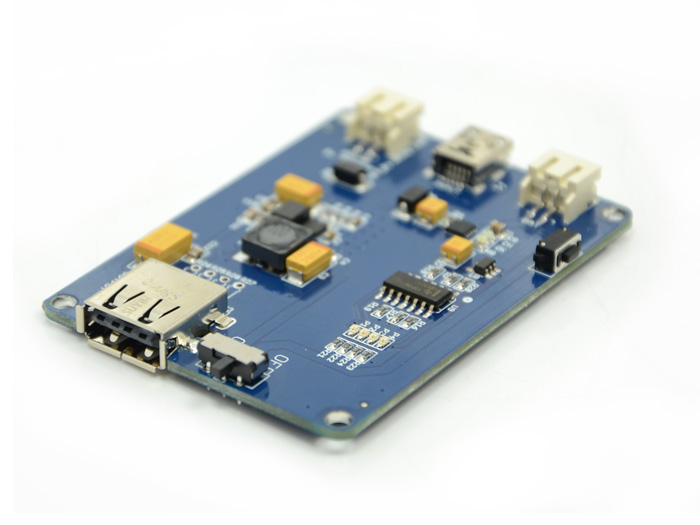
\includegraphics[width=0.5\textwidth]{./Figures/MODI/lipopro.jpg}
		\rule{35em}{0.5pt}
	\caption[lipopro1]{LiPo Rider Pro, carga de batería y boost.}
	\label{fig:lipopro1}
\end{figure}

La Lipo Rider carga una batería de Litio Polímero. Posee una alta densidad de carga, 2000mAh a 3.7V. Figura \ref{fig:bateria}
\begin{figure}[htbp]
	\centering
		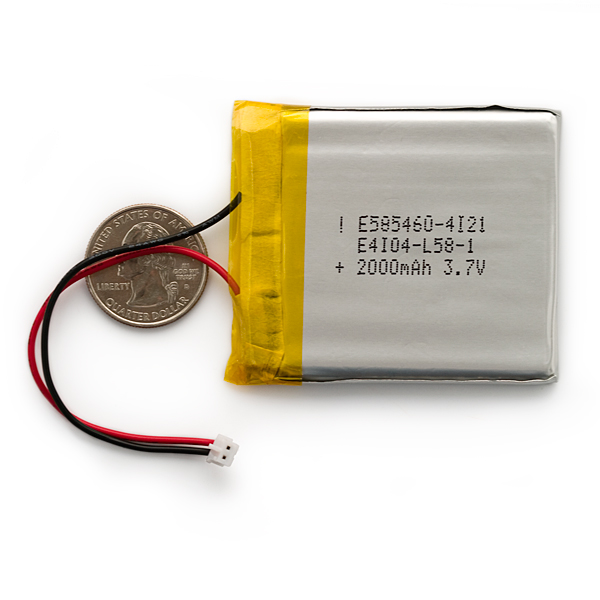
\includegraphics[width=0.5\textwidth]{./Figures/MODI/bateria.jpg}
		\rule{35em}{0.5pt}
	\caption[Bateria]{Batería lipo 2000mAh a 3.7V}
	\label{fig:bateria}
\end{figure}


%-----------------------------------
%	SUBSECTION 4
%-----------------------------------
\subsection{Motor Driver 1A Dual TB6612FNG}
El TB6612FNG motor driver puede controlar hasta dos motores DC, a una corriente constante de 1.2A (3.2A peak). Dos señales de entrada (IN1 y IN2) puede ser usadas para controlar el motor en una de cuatro modos de funcionamiento - CW, CCW, short-brake, y stop. Cada una de las salidas hacia los motores (A y B) se puede controlar separadamente, la velocidad de cada motor es controlada vía PWM con una frecuencia de hasta 100khz. El pin STBY debe colocarse en High para que el motor salga del estado Standby. Figura \ref{TB6612FNG}

\begin{figure}[htbp]
	\centering
		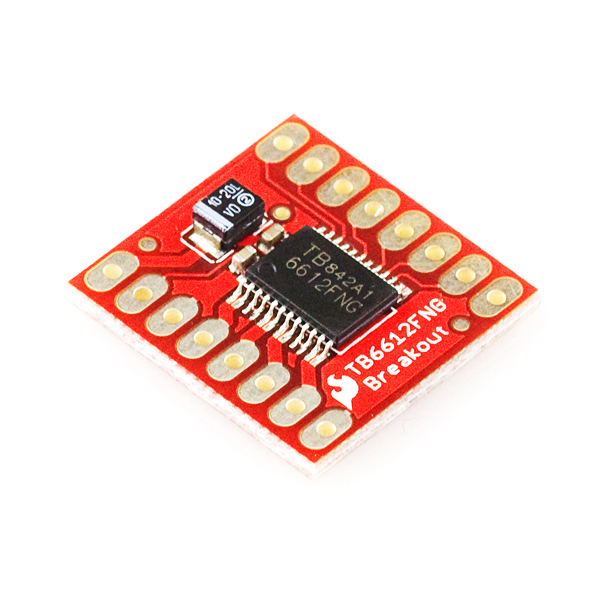
\includegraphics[width=0.5\textwidth]{./Figures/MODI/TB6612FNG.jpg}
		\rule{35em}{0.5pt}
	\caption[TB6612FNG]{Driver motores TB6612FNG.}
	\label{fig:TB6612FNG}
\end{figure}


%-----------------------------------
%	SUBSECTION 5
%-----------------------------------
\subsection{LED RGB}

LED RGB difuso, de esta manera se obtiene un ángulo de visión mucho más amplio.

Caracteristicas

Forward Voltage (RGB): (2.0, 3.2, 3.2)V \\
Max Forward Current (RGB): (20, 20, 20)mA \\
Max Luminosity (RGB): (2800, 6500, 1200)mcd

\begin{figure}[htbp]
	\centering
		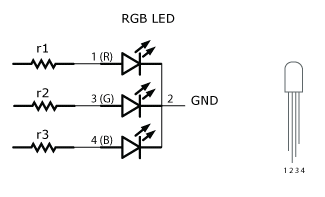
\includegraphics[width=0.5\textwidth]{./Figures/MODI/RGBLED.png}
		\rule{35em}{0.5pt}
	\caption[ledRGB]{Diagrama conexion LED RGB y resistencias por color}
	\label{fig:ledRGB}
\end{figure}

%-----------------------------------
%	SECTION 3
%-----------------------------------
\section{Componentes mecánicos}

Como se comentó en la sección \ref{cap:impresora3D}, las piezas del robot fueron diseñadas para ser construidas por una maquina de prototipado rápido del tipo FDM y se tener en cuenta la tolerancia mecánica de las piezas. En especial hay dos piezas: la rueda y el chasis, que se unen al motor. Esta unión debe quedar con un ajuste mecánico Forzado Medio \footnote{http://campuscurico.utalca.cl/\~ fespinos/Ajustes\%20y\%20tolerancias\%20mecanicas.pdf}, para que estas uniones queden fijas y las ruedas esten en el eje correspondiente.

El \textbf{Chasis} debe cumplir con la tarea de contener toda la electrónica y motores, las \textbf{Ruedas} permiten el desplazamiento y poseen dos canales para poner o-ring y así aumentar el roce con la superficie, el \textbf{Accesorio} tiene un sistema de anclaje al chasis que permite tener distintas carcasa y sensores, y el \textbf{Logo} sujeta parte de la electrónica contenida en el Chasis. 

La pieza que mas demora en construirse es el Chasis, que son 108 minutos en una Replicator 1 de MakerBot.

A continuación hay imágenes de todas las piezas renderizadas diseñadas.
\begin{figure}[htbp]
	\centering
		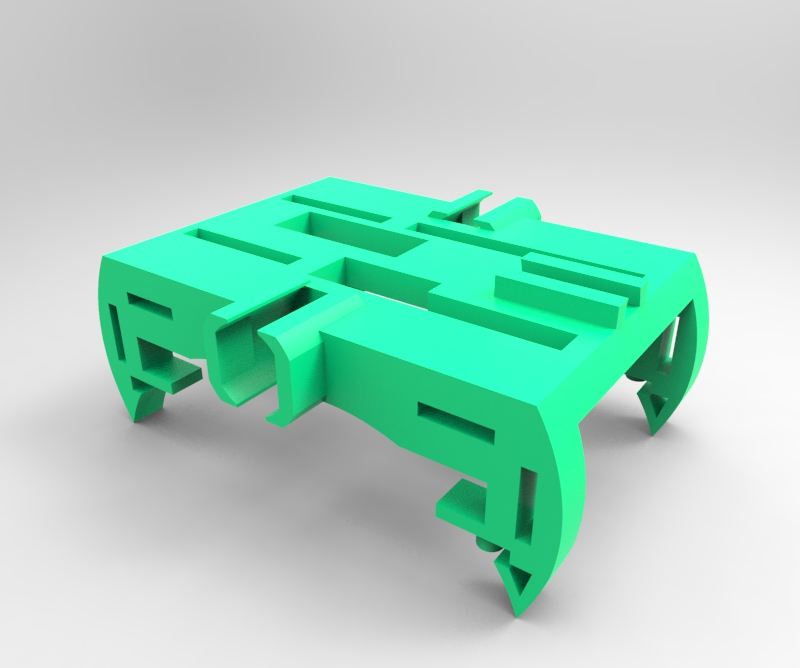
\includegraphics[width=0.8\textwidth]{./Figures/MODI/chasismodi.jpg}
		\rule{35em}{0.5pt}
	\caption[chasismodi]{Chasis modi}
	\label{fig:chasismodi}
\end{figure}

\begin{figure}[htbp]
	\centering
		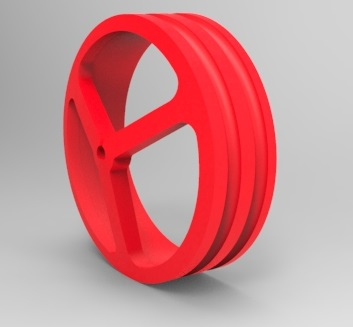
\includegraphics[width=0.8\textwidth]{./Figures/MODI/ruedamodi.jpg}
		\rule{35em}{0.5pt}
	\caption[ruedamodi]{Rueda modi}
	\label{fig:ruedamodi}
\end{figure}

\begin{figure}[htbp]
	\centering
		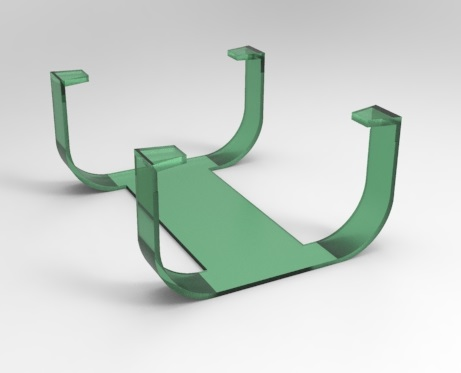
\includegraphics[width=0.8\textwidth]{./Figures/MODI/accesorio.jpg}
		\rule{35em}{0.5pt}
	\caption[accesorio]{Accesorio modi}
	\label{fig:accesorio}
\end{figure}

\begin{figure}[htbp]
	\centering
		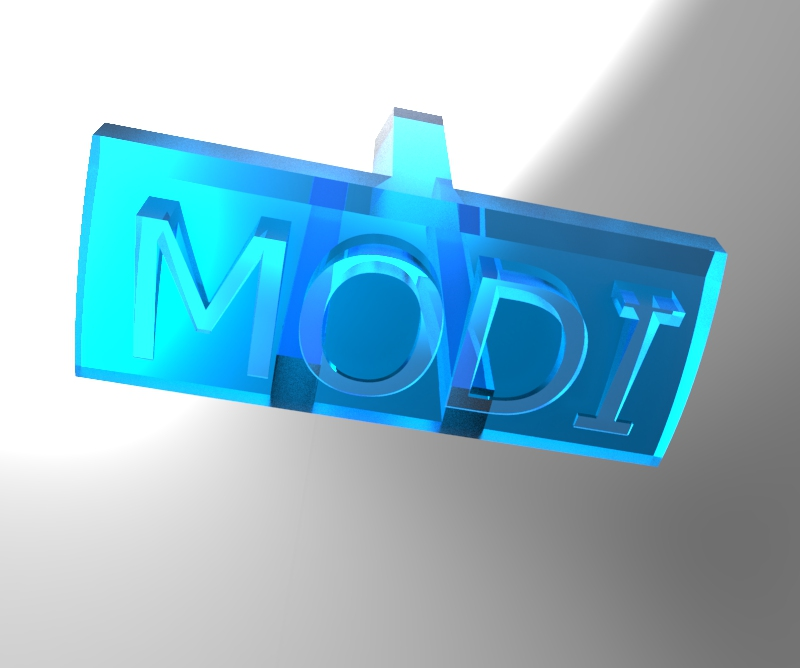
\includegraphics[width=0.8\textwidth]{./Figures/MODI/logomodi.jpg}
		\rule{35em}{0.5pt}
	\caption[logomodi]{Logo modi}
	\label{fig:logomodi}
\end{figure}

%-----------------------------------
%	SECTION 4
%-----------------------------------

\section{Locomoción}
Existen distintas áreas donde se utilizan robots, dependiendo de la tarea a realizar es la movilidad que este debe tener. Algunos tienen complejos sistemas como la plataforma del proyecto Atlas (The Agile Anthropomorphic Robot) de Boston Dynamics, Figura \ref{fig:Atlas}. En nuestro caso, solo es necesario desplazarse sobre un superficie plana y por esto, en vez de tener costosos actuadores neumáticos, la solución más simple es contar con dos motores para poder tener un movimiento diferencial. Si se desea tener más información sobre los tipos de locomoción en robots con ruedas, ver esta pagina web\footnote{en.wikibooks.org/wiki/Robotics/Types\_of\_Robots/Wheeled}.


\begin{figure}[htbp]
	\centering
		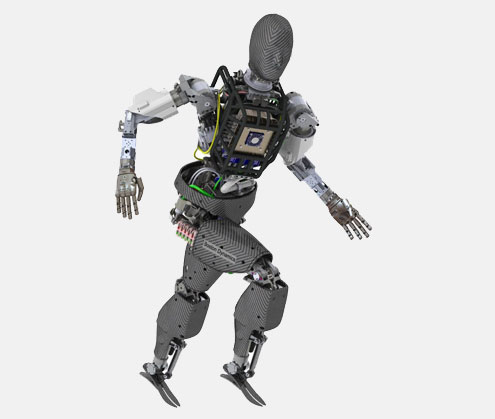
\includegraphics[width=0.5\textwidth]{./Figures/AtlasCADlr.jpg}
		\rule{35em}{0.5pt}
	\caption[Atlas]{Atlas es un humanoide con gran movilidad, diseñado para poder usar herramientas humanas. Posee 28 grados de libertad con actuadores hidráulicos y la energía se le entrega por medio de un cable flexible. Imagen extraída de bostondynamics.com }
	\label{fig:Atlas}
\end{figure}


Para moverse MODI tiene dos motores DC \ref{fig:MotorDC}. Estos tienen una caja de reducción 30:1 que permiten aumentar el torque y disminuir la velocidad. La Figura \ref{fig:DCMotor} muestra la característica de estos. 

\begin{figure}[htbp]
	\centering
		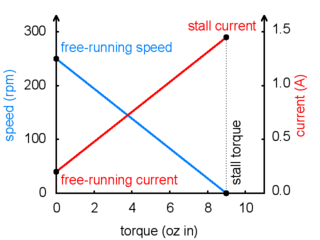
\includegraphics[width=0.5\textwidth]{./Figures/MODI/DCMotor.png}
		\rule{35em}{0.5pt}
	\caption[DCMotor]{Operación motores: Corriente, velocidad y torque. Imagen extraída de pololu.com}
	\label{fig:DCMotor}
\end{figure}

El control de velocidad de los motores se hace con pwm, que es una señal periódica a la cual se le modifica el ciclo de trabajo. El sentido de giro es controlado con el chip TB6612FNG \ref{fig:TB6612FNG}. Los valores van desde -255 a 255. Para más información sobre pwm y este chip ver esta pagina web \footnote{http://www.pololu.com/docs/0J21/5.c}.
\begin{figure}[htbp]
	\centering
		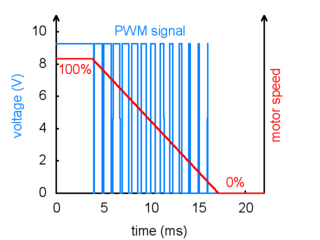
\includegraphics[width=0.5\textwidth]{./Figures/pwmchart.png}
		\rule{35em}{0.5pt}
	\caption[pwmChart]{Control de velocidad PWM, se observa como disminuye la velocidad según el ancho del pulso pwm.}
	\label{fig:pwmChart}
\end{figure}


\begin{figure}[htbp]
	\centering
		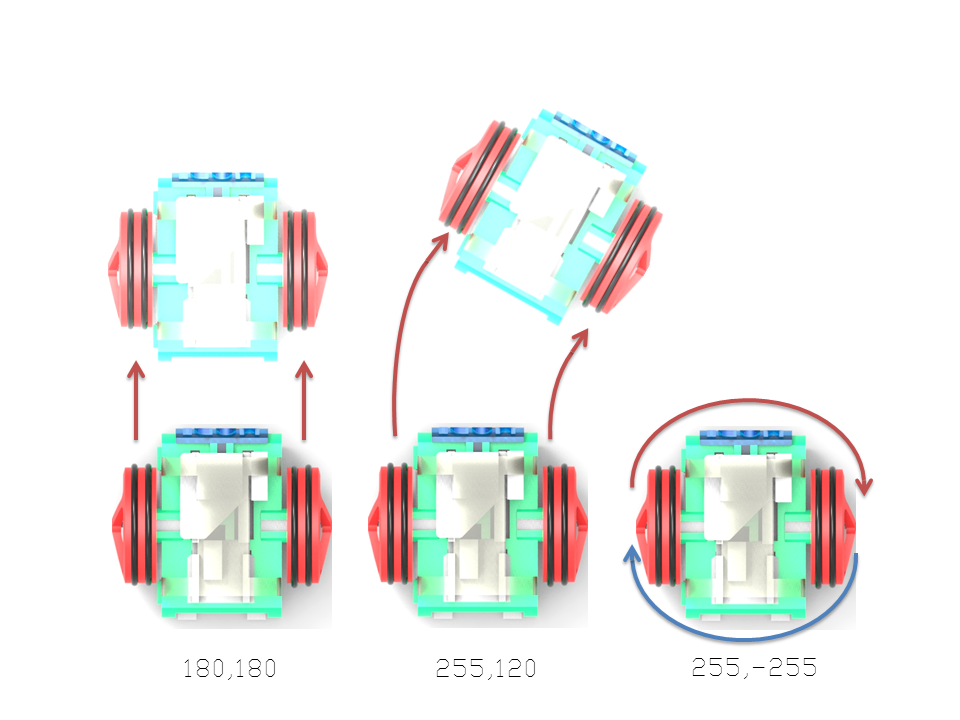
\includegraphics[width=0.8\textwidth]{./Figures/MODI/pwm.png}
		\rule{35em}{0.5pt}
	\caption[pwm]{Movimiento diferencial. A diferencia de un auto, MODI tiene dos motores que giran de forma independiente. Las distintas velocidades y sentido de giro determinan el angulo para girar. Si se necesita solamente rotar los motores deben girar en sentidos opuestos.}
	\label{fig:pwm}
\end{figure}



http://www.youtube.com/watch?v=aE7RQNhwnPQ



%-----------------------------------
%	SECTION 5
%-----------------------------------
\section{Tracking 2D}

Al igual que los seres vivos un robot necesita “sentidos” para poder tener poder interactuar con su entorno. Estos pueden ser sensores IR para detectar objetos cercanos, cámaras o LASER para hacer un mapa del entorno o simplemente un pulsador que sea presionado cada vez que el robot colisiona. Para bajar costos, MODI actualmente no cuenta con sensores “onBoard”. Cada robot es comandado por un sistema que le dice donde donde está él, dónde están los demás y los límites del área de trabajo. Se diseñó de esta manera para simplificar la programación de cada robot.

reacTIVision es un framework open source, cross-platform, para realizar tracking rápido y robusto de tags fiduciales pegadas a objetos físicos. Ha sido diseñado como un toolkit para el desarrollo rápido multi-touch interactive surfaces. Este Framework fue desarrollado por Martin Kaltenbrunner y Ross Bencina en el Music Technology Group de la universidad de Pompeu Fabra en Barcelona, España. reacTIVision fue diseñado como sensor principal de la Reactable, un sintetizador modular tangible que ha marcado los standards en lo que a aplicaciones multitouch se refiere. Esta alternativa debe ir acompañada de otros elementos, como la cámara y el computador en el cual se ejecuta el software. 


\begin{figure}[htbp]
	\centering
		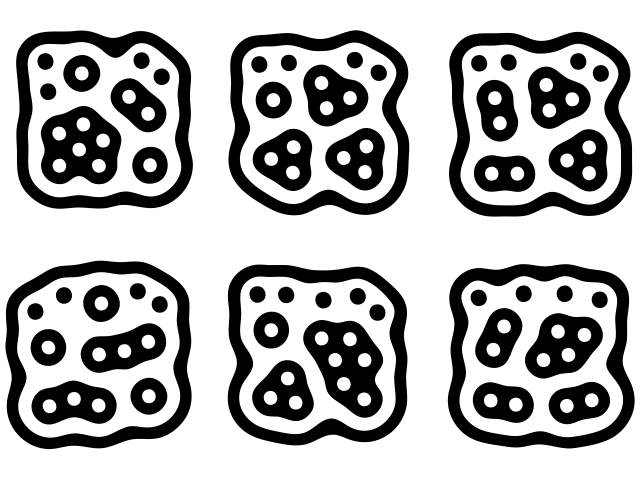
\includegraphics[width=0.8\textwidth]{./Figures/MODI/fiducial.png}
		\rule{35em}{0.5pt}
	\caption[Fiducial]{Códigos fiduciales utilizados en reacTIVision. Estos códigos aunque parecen algo extraños para los seres humanos están diseñados de tal forma que es muy fácil diferenciar unos de otros y además obtener su orientación y posición en un software de análisis de imágenes. Se tiene un total de 216 configuraciones posibles de códigos.}
	\label{fig:Fiducial}
\end{figure}

%-----------------------------------
%	SECTION 6
%-----------------------------------

\section{Software}
Software, el cerebro del robot
Gracias a un puerto serial escuchando las instrucciones para mover los motores del robot, es bastante sencillo controlar a MODI desde el computador usando cualquier lenguaje que tenga una biblioteca para uso de puertos seriales.

A continuación algunos ejemplos de como controlar a MODI. El puerto serie en MODI tiene configurada una velocidad de 115200 y esta esperando los caracteres ‘w’,’a’,’d’ y ‘s’, como Adelante, Izquierda, Derecha y Atrás respectivamente. El código de MODI, el Firmware, se encuentra en github.com/FabLabUChile/modi/


https://code.google.com/p/pytuio/
http://www.tuio.org/?software
http://pyserial.sourceforge.net/
http://www.aaronstannard.com/post/2012/08/17/How-to-Setup-a-Proper-Python-Environment-on-Windows.aspx

https://bugs.launchpad.net/python-uinput/+bug/752699


%-----------------------------------
%	SECTION 6
%-----------------------------------

\section{Bill Of Material}
http://kitbom.com/otrab/modi/build-view